%%%%%%%%%%%%%%%%%%%%%% PRELIMINARIES SECTIOn %%%%%%%%%%%%%%%%%%
\section{Preliminaries}
\label{sec:prelim}

%\begin{figure*}
%\centering
%\subfigure[{Example Topology where $v_b$ is the compromised node.}]
%{\includegraphics[width=0.49\textwidth]{figs/all-paths.pdf}}
%\subfigure[{$v_1$'s least cost paths that use $v_b$. Double slashes on an edge indicate that the edge does not actually exist 
%(but $v_b$ is claiming it has such a direct link).}]
%{\includegraphics[width=0.49\textwidth]{figs/bad-paths.pdf}}
%\caption{Motivating Example}
%\label{fig:motivate}
%\end{figure*}


%Consider the topology in Figure \ref{fig:motivate}(a) where $v_b$ is the compromised node.  In this example, $v_b$ claims it can reach every node in the graph with cost
%of $1$.  
%{\footnote {\small These edges are not shown in Figure \ref{fig:motivate}(a) because they do not actually exist.}} 
%As a result, many nodes route via $v_b$.  For example, Figure \ref{fig:motivate}(b) shows that all of $v_3$'s shortest paths that use $v_b$. Links with
%double slashes indicate distances that $v_b$ claims but are not true. The figure shows that $v_3$ uses $v_b$ to reach $v_0,v_4,v_5,v_6,v_7,$ and $v_8$.
%Specifically, to reach these nodes $v_3$ uses the paths $v_2 - v_1 - v_b - v_i$ for all $i=0,4,5,6,7,8$.  
%The example also demonstrates that $v_b$'s influence is network-wide: all nodes in this example use $v_b$ to reach multiple destinations.

%Because all nodes use $v_b$ in at least one of their least cost paths, the compromised node's influence is network-wide. 

 %For this reason we need a network-wide solution. 
\subsection{A Useful Analogy}
\label{subsec:analogy}
Before describing our recovery algorithms, we first present a useful analogy: a link cost change event in distance vector is like a distributed 
database transaction. A database transaction is a sequence of read and writes of tuples. In a distributed database these read and writes can occur over several 
different sites. Similarly, in DV a link cost change can cause a sequence of reads and writes. If the link cost change
results in a new least cost vector, update messages are sent.  Nodes that receive these update messages  \emph{read} the new distance values and update their 
distance matrix. If the received least cost vector results in a new least cost distance, a node will \emph{write} to its least cost vector and send a message, 
resulting in potentially more reads and writes. Note that we are not considering the update to the distance matrix as a \emph{write}, only
updates to the least cost vector. We use this analogy to help describe \second, \purge, and \cpr.

%Before describing our recovery algorithms, we first present a useful analogy: a link cost change event in distance vector is like a distributed 
%database transaction. A database transaction is a sequence of read and writes of tuples. In a distributed database these read and writes can occur over several 
%different sites. Similarly, in DV a \lcd can cause a sequence of reads and writes. If the \lcd
%results in a new \minv, update messages are sent.  Nodes that receive these update messages  \emph{read} the new \minv values and update their 
%distance matrix. If the received \minv results in a new least cost distance, a node will \emph{write} to its \minv and send a message, 
%resulting in potentially more reads and writes. Note that we are not considering the update to the \dmatrix as a \emph{write}, only
%updates to \minv. We use this analogy to help describe \second, \purge, and \cpr.

\subsection{Notation}
\label{subsec:notation}
In this section we define notation that we use in the next section to describe our recovery algorithms.  For each node $v \in V$, let \minv denote its least cost 
vector, \dmatrix its distance matrix, and $adj(v)$ the nodes adjacent to $v$. Let \bad denote the bad node, $t'$ the time the bad node goes bad, 
and $t$ the time the bad node is discovered. We assume that when a node is discovered to be at $t$ the value of $t'$ is known.
The bad node's least cost vector before going bad is denoted \oldvectors, while its least cost value after it has gone bad is \badvectors.
Finally, we use \lcd to denote the value of the link cost change when a link cost change event occurs.

%%%%%%%%%%%%%%%% BEGIN COMMENT %%%%%%%%%%%%%%%%%%%%%%%%%
\begin{comment}
\begin{figure*}[t]
\begin{center}

\begin{tikzpicture}
	\word[6cm]{\wordu}{}
	%\word[0cm]{\wordv}{}
	\dwordpos{5cm}{$t$}
	\dwordpos{1cm}{$t'$}
	\dwordpos{1cm}{$t'$}
	%\dwordposhack{1cm}{$g$}{}
	%\draw[decorate,decoration=brace] ($t'$) -- ($t$);	
	%\wordupoint{5cm}{$x$}
	%\wordvpoint{3cm}{$x$}
	%\wordupoint{4cm}{$S:y$}
	%\wordvpoint{1cm}{$D:y$}
\end{tikzpicture}
\end{center}
\caption{Timing of events}
\label{fig:setup}
\end{figure*}

\end{comment}
%%%%%%%%%%%%%%%% END COMMENT %%%%%%%%%%%%%%%%%%%%%%%%%

Table \ref{tab:abbrev} summarizes the notational shorthand used in this document.

\begin{table}[h]
\begin{center}
\begin{tabular}{l l} 
\hline \hline
   	{\bf Abbreviation} & {\bf Meaning} \\
		  \hline 
			\minv & the least cost vector for each node \\
			\dmatrix & the distance matrix for each node* \\ 
			\lcd & link cost change \\
			DV & Distance Vector \\
			\hline
			$t$ & the time the oracle detects the bad node \\
			$t'$ & the time the bad node ``went bad'' \\
			\badvector & the bad node's least cost vector at and after $t$  \\
			\oldvector & the bad node's least cost vector at and before $t'$ \\
			\bad & the bad node \\ 
			$adj(v)$ & nodes adjacent to $v$  \\ 
			\hline \hline
			\end{tabular}
			\end{center}
			\caption{Table of abbreviations}
\label{tab:abbrev}
\end{table}

* The distance matrix for node $v$ contains $v$'s distance to all nodes $v_d \in V$ via all $v_n: v_n \in adj(v)$.


\begin{center}
\begin{picture}(21,2)(-10,0)
\numbline[1]{-10}{11}
\numbline{-75}{125} 
\put(125,0){\sethlabel{t}} 

\end{picture} 
\end{center}


%{\it Comment: think it would be useful to have a simple diagram like the one i have been using to draw $t$ and $t'$}

